\documentclass[11pt, a4paper]{article}
\usepackage[margin=1in]{geometry}

\usepackage{graphicx}
\newcommand{\executeiffilenewer}[3]{
	\ifnum\pdfstrcmp{\pdffilemoddate{#1}}
	{\pdffilemoddate{#2}}>0
	{\immediate\write18{#3}}\fi
}
\newcommand{\includesvg}[1]{
	\executeiffilenewer{#1.svg}{#1.pdf}
	{inkscape -D #1.svg -o #1.pdf --export-latex}
	\input{#1.pdf_tex}
}

\usepackage[utf8]{inputenc}
\usepackage[portuguese]{babel}
\usepackage{csquotes}

\usepackage{hyperref}
\usepackage{biblatex}
\addbibresource{referencias.bib}

\usepackage[shortlabels]{enumitem}

\usepackage{mathtools}
\usepackage{amssymb}
\usepackage{commath}
\newcommand{\R}{\mathbb R}

\begin{document}

%%%%%%%%%%%%%%%%%%%%%%%%%%%%%%%%%%%%%%%%%
% Academic Title Page
% LaTeX Template
% Version 2.0 (17/7/17)
%
% This template was downloaded from:
% http://www.LaTeXTemplates.com
%
% Original author:
% WikiBooks (LaTeX - Title Creation) with modifications by:
% Vel (vel@latextemplates.com)
%
% License:
% CC BY-NC-SA 3.0 (http://creativecommons.org/licenses/by-nc-sa/3.0/)
% 
% Instructions for using this template:
% This title page is capable of being compiled as is. This is not useful for 
% including it in another document. To do this, you have two options: 
%
% 1) Copy/paste everything between \begin{document} and \end{document} 
% starting at \begin{titlepage} and paste this into another LaTeX file where you 
% want your title page.
% OR
% 2) Remove everything outside the \begin{titlepage} and \end{titlepage}, rename
% this file and move it to the same directory as the LaTeX file you wish to add it to. 
% Then add \input{./<new filename>.tex} to your LaTeX file where you want your
% title page.
%
%%%%%%%%%%%%%%%%%%%%%%%%%%%%%%%%%%%%%%%%%

%----------------------------------------------------------------------------------------
%	TITLE PAGE
%----------------------------------------------------------------------------------------

\begin{titlepage} % Suppresses displaying the page number on the title page and the subsequent page counts as page 1
	\newcommand{\HRule}{\rule{\linewidth}{0.5mm}} % Defines a new command for horizontal lines, change thickness here
	
	\center % Centre everything on the page
	
	%------------------------------------------------
	%	Headings
	%------------------------------------------------

	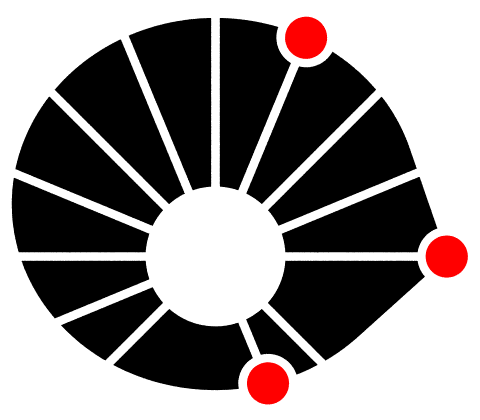
\includegraphics[width=0.2\textwidth]{unicamp_logo.png}\\[1cm] % Include a department/university logo - this will require the graphicx package
	
	\textsc{\LARGE Universidade Estadual de Campinas}\\[1.5cm] % Main heading such as the name of your university/college
	
	\textsc{\Large Instituto de Matemática, Estatística e Computação Científica}\\[0.5cm] % Major heading such as course name
	
	\textsc{\large MS211 - Calculo Numérico}\\[0.5cm] % Minor heading such as course title
	
	%------------------------------------------------
	%	Title
	%------------------------------------------------
	
	\HRule\\[0.4cm]
	
	{\huge\bfseries Relatório - Projeto SIR}\\[0.4cm] % Title of your document
	
	\HRule\\[1.5cm]
	
	%------------------------------------------------
	%	Author(s)
	%------------------------------------------------
	
	%\begin{minipage}{0.6\textwidth}
		\begin{flushleft}
			\large
			\textit{Alunos}\\
			Guido Neulaender - 217100 \\
			Heloisa Pimentel Lins de Silva - 236510 \\
			João Francisco Figueiredo Miranda - 218592 \\
			Rodrigo Ryan Oliveira da Silva - 244024 \\
			Silas Leonel Pereira Miranda - 258984
		\end{flushleft}
	%\end{minipage}
	~
	
	% If you don't want a supervisor, uncomment the two lines below and comment the code above
	%{\large\textit{Author}}\\
	%John \textsc{Smith} % Your name
	
	%------------------------------------------------
	%	Date
	%------------------------------------------------
	
	\vfill\vfill\vfill % Position the date 3/4 down the remaining page
	%\begin{minipage}{0.4\textwidth}
		\begin{flushright}
			\large
			\textit{Professor}\\
			Dr. Maicon Ribeiro Corrêa % Supervisor's name
		\end{flushright}
	%\end{minipage}
	
	{\large\today} % Date, change the \today to a set date if you want to be precise
	
	%------------------------------------------------
	%	Logo
	%------------------------------------------------
	 
	%----------------------------------------------------------------------------------------
	
	\vfill % Push the date up 1/4 of the remaining page
	
\end{titlepage}


Esse projeto foi feito com intuito de compreender a evolução do coronavírus no Estado de Minas Gerais.
Nele foi utilizado o modelo compartimental SIR (Suscetíveis-Infectados-Removidos), que divide a população (N) em 3 grupos: suscetíveis a infecção (S); os que já foram infectados e que podem infectar os  (I); e os que já foram removidos (R), seja por terem sido curados ou pelo óbito. 
É sabido que esses 3 grupos interagem segundo o seguinte sistema de Equações Diferenciais Ordinárias (EDOs):
\[
	\od{S}{t} = - \gamma r_0 \frac{IS}{N} , \quad
	\od{I}{t} = \gamma \left( r_0 \frac{IS}{N} - I \right) \text{ e} \quad
	\od{R}{t} = \gamma I
\]
onde $r_0 = \frac{\beta}{\gamma}$ é constante ou dado em função do tempo. 
Para simulação desse sistema foi utilizado o método numérico de Runge-Kutta, que foi escolhido por ser um método bastante flexível, o que permite que sejam simulados  diversos cenários com diversas condições iniciais.
Vale ressaltar que foram utilizadas como base de dados as seguintes referências:
o painel coronavírus, organizado pelo Professor Alberto Saa \cite{painel_covid};
o site da Wikipédia sobre \emph{Compartmental models in epidemiology} \cite{model}
e o livro Cálculo Numérico de Marcia A. G. Ruggiero e Vera L. R. Lopes \cite{calc_num}.
Ao final da pesquisa, conseguimos obter alguns resultados, disponibilizados em anexo ao final do relatório, que iremos discutir brevemente o que eles querem dizer e com toda implementação do código podendo ser encontrada no GitHub do grupo \cite{git_grupo}.

Para compreensão da evolução do coronavírus a partir do sistema de EDOs, dito anteriormente, foi-se avaliada duas possibilidades em relação ao $r_0$, a primeira com o seu valor constante e a segunda com seu valor variando em relação ao tempo.
Possivelmente, a principal diferença entre as duas possibilidades deve-se ao fato de que a segunda terá valores mais exatos do que a primeira, já que ela estará mudando sempre com o tempo devido a variação da taxa de infecção, enquanto a primeira terá sempre o mesmo valor independente das condições.

Para a primeira possibilidade, em que o $r_0$ é dito constante, adotamos seu valor como $r_0 \approx 2,6$, dado pela simples razão entre a taxa de infecção ($\beta \approx 0,34$) e a taxa de remoção ($\gamma \approx 0,13$).
Já a segunda possibilidade, que seria o $r_0$ em função do tempo, foi calculado a partir da seguinte fórmula, dados $\gamma$ e $\alpha$:
\[
	r_0(t) = \frac{1}{1 - \mu} + \frac{\ddot{C}}{\gamma \dot{C} (1 - \mu)}
	\text{, com} \quad
	\mu(t) = \frac{\alpha}{\gamma N} (\gamma C + \dot{C})
\]
sendo $C$ o número de casos acumulados até o dia $t$, $\dot{C}$ são o número de casos novos e
$\ddot{C}$ é a variação do crescimento dos casos.
A constante $\alpha$ (entre $10 < \alpha < 20$) é uma estimativa da relação entre o valor real $R$ de indivíduos removidos e o número de casos acumulados, isto é, $R = \alpha C$.
Tendo feito isso percebemos que o gráfico dos casos novos estava com muitos ruídos, principalmente pelo atraso dos diagnósticos, e para solucionar esse problema fizemos uma suavização do gráfico utilizando o filtro de média móvel:
\[
	\overline{C}_t = \frac{1}{2n+1} \sum_{k=t-n}^{t+n} C_k
\]
onde $n$ delimita uma vizinhança simétrica de tamanho $2n+1$ em volta de um termo $C_t$.
No nosso caso, seguimos o mesmo procedimento adotado em "Análise automática do Painel Coronavírus" do Prof. Alberto Saa \cite{pdf_saa}, aplicando uma suavisação de $n=3$ quatro vezes.
Para tanto, usamos a seguinte extensão de dados em cada uma das aplicações
\[
	C_{1-j} = C_1
	\quad \text{e} \quad
	C_{k+j} = C_k + C_{k-n+j} - C_{k-n},
\]
adicionando $2n$ novos elementos para não perdemos dados após a aplicação do filtro.
Finalmente obtida uma suavisação satisfatória para o gráfico, calculamos os valores de $r_0$ e pudemos substituir seu valor no sistema de EDOs para ambas as possibilidades e finalmente aplicamos o método de Runge-Kutta, com a simulação podendo ser encontrada em anexo ao final do relatório.

Com $r_0$ constante, e iniciando a partir de um dia onde haviam 7 casos no estado de Minas Gerais, 17 de março de 2020, e usando como período total da incidência do vírus em torno de 140 dias, chegamos ao gráfico que está no anexo 3. Nele, podemos perceber que com o avanço do vírus no estado, o grupo de infectados, aumenta abruptamente tendo um pico em torno de 70 dias e, após o dobro de tempo, tende a zero.
qui, podemos perceber  que o vírus tende a rapidamente atingir um grande número de pessoas, fazendo o número de pessoas suscetíveis a infecção diminuir junto com o aumento de infectados, tendendo zero. Ainda, o número de removidos, aumenta a partir do ápice de infectados, mostrando que caso a doença acometer quase toda a população em pouco tempo teria um número de removidos maior que o de infectados.

Esta simulação mostra um cenário onde há a ausência da prevenção do vírus.
Neste caso, rapidamente haveria um enorme número de infectados atingindo milhares de pessoas em poucos dias.
E, também, o número de removidos, por considerar além de pessoas curadas e imunes ao vírus, considera também o número de óbitos, ou seja, não se sabe ao certo a porcentagem da população que criou imunidade ao vírus e a que não resistiu.
Isso mostra que num quadro assim, poderiam haver danos irreparáveis à população geral.

Visando entender melhor a evolução efetiva do vírus, avaliamos como $r_0$ varia com o tempo fazendo, a partir dos dados disponíveis na referência \cite{model}
fizemos um ajuste da curva do $r_0(t)$
usando um decaimento exponencial visto que a curva do $r_0(t)$
tende a se aproximar do eixo das abscissas, portanto o decaimento exponencial pareceu ser mais coerente com esse comportamento.
Para isso usamos um decaimento de primeira ordem em que a equação é da forma
\[
	r_0(t) = y_0 + A e^{-t/c}
\]
e substituindo pelos coeficientes
\[
	r_0(t) = 1,282 + 3,566 e^{-t/7,809},
\]
com isto plotamos o gráfico disponível no anexo 4.

Ao comparar o os resultados das simulações observamos que A curva simulada com $r_0$
fixo tem uma menor incidência, fazendo com que a doença tenha um ápice muito rápido e que rapidamente acomete grande parte da população.
Já no caso do $r_0$ variável a doença demora mais para atingir o máximo de infectados ao mesmo tempo e, além de ficar mais tempo com esse máximo, ainda acomete um menor número de infectados ao mesmo tempo (neste caso, 10 vezes menos).
As curvas de removidos e suscetíveis, R e S respectivamente, também diferem muito nos dois casos, diferente do primeiro caso, o segundo o R se se mantém alto durante todo o tempo de incidência, caindo apenas pela metade durante o período simulado.
Também o número de removidos tende a ser menor.
Como juntos com os removidos temos os óbitos, o número total de óbitos no caso 2 pode ser bem menor que no caso 1.

Avaliando dois casos, um onde a incidência do vírus ocorre num curto período do tempo mas que há um enorme número de infectados ao longo do tempo, e outro onde o vírus incide por um tempo maior, há um menor número de infectados ao longo do tempo e um possível menor número de mortes no total, vemos que o segundo caso é menos prejudicial ao estado que o primeiro.
Ainda, por se aproximar do real avanço do vírus no estado, ao avaliar o segundo caso estamos também avaliando as medidas de proteção tomadas pelos indivíduos, que é quase nula no primeiro.
Ressaltamos ainda que ambas as simulações têm a mesma data incial mas a incidência do vírus se faz diferente nos dois casos.

Por fim, podemos perceber, ao compreender a evolução do vírus em minas gerais que ela acontece não tão rapidamente e com um ápice que tende a levar mais de 100 dias para haver uma queda.
O número total de retirados tende a metade do total populacional estudado, mostrando que ao menos metade da população, se não imune, vai contrair o novo coronavírus.

O método numérico implementado se faz eficiente para o estudo do avanço do vírus, e a parte matemática auxilia na simulação. ainda, conseguimos a partir do avanço real do vírus simular um quadro que mostra previsões para o avanço dele ao longo dos próximos dias utilizando apenas do ferramental do método.
Ademais, podemos perceber que modelos que matemáticos podem auxiliar na resolução de diversos problemas nas mais diversas áreas da ciência, mostrando a importância da matemática e do estudo científico para a população geral.

\newpage
\section*{Anexos}
\begin{enumerate}[1.]
	\item Dados preliminares do coronavírus no Brasil.
	\begin{figure}[h]
		\centering
		\textbf{Brasil}\par\medskip
		\scalebox{.7}{\includesvg{BR_r0-aprox}}
	\end{figure}

	\item Dados preliminares do coronavírus em Minas Gerais.
	\begin{figure}[h]
		\centering
		\textbf{Minas Gerais}\par\medskip
		\scalebox{.7}{\includesvg{MG_r0-aprox}}
	\end{figure}

	\newpage
	\item Simulação com $r_0$ constante.
	\begin{figure}[h]
		\centering
		\scalebox{.8}{\includesvg{sim_r0fixo}}
	\end{figure}

	\item Simulação com $r_0$ variando.
	\begin{figure}[h]
		\centering
		\scalebox{.8}{\includesvg{sim_r0variavel}}
	\end{figure}

	\newpage
	\item Ajuste exponencial da curva do $r_0(t)$ em Minas Gerais no SciDAVis.
	\begin{figure}[h]
		\centering
		\scalebox{.6}{\includesvg{ajuste_r0}}
	\end{figure}

	\item Aplicação do método de Runge-Kutta no sistema de EDOs.
	
	Nós sabemos resolver pelo método de Runge-Kutta PVIs da forma
\[
	\left\{ \begin{array}{ll}
	y' &= f(x,y) \\
	y(x_{0}) &= y_{0}
	\end{array} \right.
\]
usando a formula de quarta ordem:
\[
	\begin{split}
	y_{n+1} &= y_n + \frac{1}{6} \left( k_1 + 2 k_2 + 2 k_3 + k_4 \right)
	, \quad \text{onde} \\
	k_1 &= \Delta x \cdot f(x_n, y_n) \\
	k_2 &= \Delta x \cdot f(x_n + \Delta x / 2, y_n + k_1 / 2) \\
	k_3 &= \Delta x \cdot f(x_n + \Delta x / 2, y_n + k_2 / 2) \\
	k_4 &= \Delta x \cdot f(x_n + \Delta x , y_n + k_3 )
	\end{split}
\]

Precisamos, então, reescrever as equações do modelo SIR
\[
	\od{S}{t} = - \gamma r_0 \frac{IS}{N} , \quad
	\od{I}{t} = \gamma \left( r_0 \frac{IS}{N} - I \right) \text{ e} \quad
	\od{R}{t} = \gamma I
\]
de forma que consigamos aplicar Runge-Kutta. Para isso, vamos vetorizar!
\[
	\vec{u} = \left( \begin{array}{rr}
	S \\
	I \\
	R
	\end{array} \right) \text{ e } \quad
	\vec{f}(t,\vec{u}) = \left( \begin{array}{rr}
	f_1 \\
	f_2 \\
	f_3
	\end{array} \right) \text{, com} \quad
	f_1 = - \gamma r_0 \frac{IS}{N} , \quad
	f_2 = \gamma \left( r_0 \frac{IS}{N} - I \right) \text{ e} \quad
	f_3 = \gamma I
\]
Dessa forma temos que
\[
	\od{\vec{u}}{t} = \vec{f}(t, \vec{u}) \text{ e} \quad
	\vec{u}(t_0) = u_0
\]
e portanto podemos aplicar Runge-Kutta:
\[
	\begin{split}
	\vec{u}_{n+1} &= \vec{u}_n + \frac{1}{6} \left( \vec{k}_1 + \vec{2 k}_2 + \vec{2 k}_3 + \vec{k}_4 \right)
	, \quad \text{onde} \\
	\vec{k}_1 &= \Delta t \cdot f(t_n, \vec{u}_n) \\
	\vec{k}_2 &= \Delta t \cdot f(t_n + \Delta t / 2, \vec{u}_n + k_1 / 2) \\
	\vec{k}_3 &= \Delta t \cdot f(t_n + \Delta t / 2, \vec{u}_n + k_2 / 2) \\
	\vec{k}_4 &= \Delta t \cdot f(t_n + \Delta t , \vec{u}_n + k_3 )
	\end{split}
\]


	
\end{enumerate}
\printbibliography

\end{document}

